%------------------------------------------
% Este é o estilo/template de formatação de 
% TCC 2 no formato de artigo do DCC/UFRR.
% Este documento utiliza como base o modelo
% de formatação da SBC (Sociedade Brasileira
% de Computação). Disponivel em: 
% https://www.sbc.org.br/wp-content/uploads/2024/07/modelosparapublicaodeartigos.zip
%------------------------------------------

\documentclass[12pt]{article}

% --------------------------------------
% Pacotes utilizados 
% --------------------------------------
\usepackage{estilo/sbc-template}
\usepackage{tikz}
\usepackage{transparent}
\usepackage{graphicx,url}
\usepackage[utf8]{inputenc}
\usepackage[brazil]{babel}
\usepackage{todonotes}
\usepackage{fancyhdr}
\usepackage{multirow}
\usepackage{scalefnt}
\usepackage{float}
\usepackage{datetime}
\usepackage{ifthen}
\usepackage[alf]{abntex2cite} 
\usepackage{listings}
\usepackage{subcaption}
\usepackage{bigstrut}
\usepackage{array}


% --------------------------------------
% Configurações de formatação de código
% --------------------------------------
\lstset
{ %Formatting for code
    language=C,
    basicstyle=\footnotesize,
    numbers=left,
    stepnumber=1,
    frame = single,
    showstringspaces=false,
    tabsize=2,
    breaklines=true,
    xleftmargin=10pt,
    breakatwhitespace=false,
    extendedchars=true,
    literate={á}{{\'a}}1 
             {ã}{{\~a}}1
             {é}{{\'e}}1
             {í}{{\'i}}1
             {õ}{{\~o}}1
             {ç}{{\c{c}}}1,
}


% --------------------------------------
% Definições de formatação
% Númeração das páginas
% --------------------------------------
\pagestyle{fancy}
\fancyhf{}
\fancyhead[R]{\thepage}
\renewcommand{\headrulewidth}{0pt}


\sloppy

% --------------------------------------
% Definições de informações do TCC
% --------------------------------------
\title{TÍTULO DO TRABALHO}

\author{NOME DO DISCENTE}

\orientador{Prof. Título. Nome Completo}
% Caso não tenha coorientador, deixar o campo vazio.
\coorientador{}
% Caso tenha coorientador, descomentar linha abaixo.
%\coorientador{Prof. Título. Nome Completo}

\address{
  Curso de Bacharelado em Ciência da Computação\\ 
  Departamento de Ciência da Computação\\ 
  Universidade Federal de Roraima (UFRR)\\ 
  Boa Vista -- RR -- Brasil  
  \email{\{aluno\}@ufrr.br}
}

% Caso não tenha agradecimentos, deixar o campo vazio.
\agradecimento{
  \todo[inline]{É opcional, mas é comum que se escreva esta seção de modo a reconhecer as pessoas e organizações que contribuíram de modo relevante com o desenvolvimento da pesquisa até a etapa de qualificação, como o(a) orientador(a), os docentes do PPCA, os colegas de grupo de pesquisa e a instituição em que o(a) discente atua profissionalmente. Caso a pesquisa tenha recebido bolsa ou financiamento, é obrigatório agradecer à agência de fomento; para apoio da CAPES, utilize o texto previsto na Portaria CAPES nº 206/2018: ``O presente trabalho foi realizado com apoio da Coordenação de Aperfeiçoamento de Pessoal de Nível Superior -- Brasil (CAPES) -- Código de Financiamento 001''. Exemplo: Ao meu orientador, pela condução criteriosa desta pesquisa, e aos docentes do Programa de Pós-Graduação em Computação Aplicada, pelas contribuições que aproximaram este trabalho dos desafios reais da minha prática profissional.}
}
% --------------------------------------


% --------------------------------------
% Início do documento
% --------------------------------------
\begin{document} 

% Não é necessário alterar
% Capa personalizada para UFRR
\begin{titlepage}
    \begin{tikzpicture}[remember picture,overlay]
        \node[opacity=0.1,inner sep=0pt] at (current page.center){
            
\includegraphics[width=0.9\paperwidth]{estilo/logo-ppca.png}
        };
    \end{tikzpicture} 

    \begin{center}
        % Imagem no topo (troque o nome do arquivo para o correto)
        
\includegraphics[width=0.2\textwidth]{estilo/ufrr-logo.png} %\\[2cm]

        % Instituição
        {\large
        UNIVERSIDADE FEDERAL DE RORAIMA\\
        CENTRO DE CIÊNCIAS E TECNOLOGIA\\
        PROGRAMA DE PÓS-GRADUAÇÃO EM COMPUTAÇÃO APLICADA\\[3cm]
        }

        % Nome do aluno
        {\bfseries\Large 
            \makeatletter
            \@author
            \makeatother
        }\\[1.5cm]

        % Título do trabalho
        {\bfseries\LARGE 
            \makeatletter
            \@title
            \makeatother
        }

        \vfill

        % Data
        {\large Boa Vista - RR\\
        \today}
    \end{center}
\end{titlepage}

% Folha de rosto
%\newpage
\begin{titlepage}
    \begin{tikzpicture}[remember picture,overlay]
        \node[opacity=0.1,inner sep=0pt] at (current page.center){
            
\includegraphics[width=0.9\paperwidth]{estilo/logo-ppca.png}
        };
    \end{tikzpicture}
    \begin{center}
        % Título em negrito no topo
        {\bfseries\LARGE 
            \makeatletter
            \@title
            \makeatother
        }\\[4cm]

        % Nome do discente
        {\Large 
            \makeatletter
            \@author
            \makeatother
        }\\[4cm]

        % Texto com recuo à direita
        \begin{flushright}
            \parbox{9cm}{\setlength{\parindent}{0pt}
            Texto de Qualificação apresentado ao Programa de Pós-Graduação em Computação Aplicada (PPCA) da Universidade Federal de Roraima, na modalidade Mestrado Profissional, como requisito parcial para a obtenção do título de Mestre em Computação Aplicada.
            }
        \end{flushright}

        \begin{flushright}
            \parbox{9cm}{\setlength{\parindent}{0pt}
            \textbf{Orientador:} \getorientador.
            }
        \end{flushright}
        
        \ifcoorientadordefined{
            \begin{flushright}
                \parbox{9cm}{\setlength{\parindent}{0pt}
                \textbf{Coorientador:} \getcoorientador.
                }
            \end{flushright}
        }

        \vfill

        % Data ao final da página
        {\large Boa Vista - RR\\
        \today}
    \end{center}
\end{titlepage}

\ifagradecimentodefined{
  %------------------------------------------
% Agradecimentos
% Este arquivo contém o conteúdo da página de agradecimentos do TCC.
%------------------------------------------
\begin{titlepage}
    \begin{tikzpicture}[remember picture,overlay]
        \node[opacity=0.1,inner sep=0pt] at (current page.center){
            
\includegraphics[width=0.9\paperwidth]{estilo/logo-ppca.png}
        };
    \end{tikzpicture}
    \begin{center}
        % Título em negrito no topo
        {\bfseries\LARGE AGRADECIMENTOS}\\[4cm]

        
        % Texto de Agradecimentos        
        {\bfseries\Large \getagradecimento}

        

        \vfill

        % Data ao final da página
        {\large Boa Vista - RR\\
        \today}
    \end{center}
\end{titlepage}

}

% Alterar após a aprovação da defesa de TCC 2
\begin{titlepage}

    \begin{center}
    \textcolor{red}{[PÁGINA PARA INSERÇÃO DA FICHA CATALOGRÁFICA]}

    \textcolor{red}{Este documento será um pdf disponibilizado pela biblioteca da ufrr ao final do seu tcc 2. Para isso, você precisará enviar o seu tcc 2 em pdf para o e-mail processamento.tecnico@ufrr.br para mais informações, consulte  https://ufrr.br/bibliotecas/elaboracao-de-ficha-catalografica . O pdf recebido será uma página. você poderá converter em imagem e inserir aqui ou, tendo o seu tcc 2 em pdf, é só inserir essa página adicional a partir de um software editor de pdf.}
    \end{center}

\end{titlepage}
\begin{titlepage}

    \begin{center}
    \textcolor{red}{[PÁGINA PARA INSERÇÃO DA ATA DE APROVAÇÃO DA QUALIFICAÇÃO]}

    \textcolor{red}{A ata do exame de qualificação é lavrada pela banca no dia do exame e arquivada pela secretaria do PPCA. Na versão final da qualificação, após a defesa, esta página receberá a folha de aprovação assinada pelos membros da banca, em PDF de uma página disponibilizado pelo(a) orientador(a) ou pela secretaria do programa. Ao receber o arquivo, basta inseri-lo aqui.}
    \end{center}

\end{titlepage}

% --------------------------------------
% Sumário
% --------------------------------------
\renewcommand{\contentsname}{\centering \bfseries SUMÁRIO}
\tableofcontents
\thispagestyle{empty}

\clearpage
\pagenumbering{arabic}
\maketitle

% --------------------------------------
% Resumo em português
% --------------------------------------
\begin{resumo} 
  \textcolor{red}{Comece com uma sentença apresentando o objetivo do estudo. Depois descreva o método. Passe para uma breve descrição de resultados, indicando, então, a conclusão do seu estudo. Finalize com uma frase que pode, por exemplo, convidar a comunidade científica para realizar mais estudos semelhantes ao seu ou que indique a contribuição do seu trabalho. O seu resumo deve ter, no máximo, 150 palavras ou 10 linhas. O mesmo vale para o abstract. Importante: em um resumo, tipicamente, não fazemos citações. Além disso, não se deve inserir fórmulas, equações, diagramas ou símbolos.}
\end{resumo}


% --------------------------------------
% Resumo em inglês
% --------------------------------------
\begin{abstract}
  \textcolor{red}{Dica para a produção de um resumo em inglês: traduza o texto em português com a ajuda do Google Tradutor. Depois use uma versão gratuita do Grammarly para avaliar a qualidade do texto. Aceite as sugestões desse software.}
\end{abstract}


% --------------------------------------
% Keywords do artigo
% --------------------------------------
\keywords{Word 1, Word 2, Word 3}


%--------------------------------------
% Seções do artigo
%--------------------------------------
%------------------------------------------
% Título: Introdução
%------------------------------------------
\section{Introdução}
\label{sec:introducao}


\todo[inline]{\textbf{NOTA}: O texto aqui apresentado contém apenas orientações para a escrita do seu texto de qualificação e DEVE SER REMOVIDO.}

\textcolor{red}{A função da introdução é apresentar à banca o tema da pesquisa, delimitar o problema investigado e demonstrar a sua relevância científica, tecnológica e/ou social, sendo finalizada com a descrição de como o texto está organizado. No exame de qualificação, a introdução deve permitir que a banca avalie, logo de início, se o problema é pertinente, se os objetivos são exequíveis no prazo restante do mestrado e se a pesquisa possui aderência à área de concentração e à linha de pesquisa do PPCA. Por se tratar de um Mestrado Profissional, é essencial evidenciar a aplicabilidade do trabalho: o contexto real (organização, setor ou comunidade) em que o problema se manifesta e o produto técnico ou tecnológico esperado como resultado (por exemplo, software, aplicativo, processo, protocolo, base de dados, relatório técnico). Apesar de ser a primeira seção, normalmente é a última a ser revisada, pois só apresentamos aquilo que já escrevemos.}

\textcolor{red}{1) Comece com uma sentença descrevendo o tema da pesquisa e o que você pretende investigar. 2) Na sequência, apresente brevemente o estado atual do tema e passe para a motivação da pesquisa. Motivos são argumentos, isto é, justificativas que indicam por que a pesquisa é necessária. Argumente, preferencialmente, com base em dados e evidências da literatura ou do contexto profissional em que o problema ocorre, indicando a lacuna que o trabalho pretende preencher. O ideal é ter de dois a três argumentos, sustentados por citações, que mostrem a relevância do tema para a ciência e o impacto esperado para a sociedade ou para o setor produtivo.}

\textcolor{red}{3) Explicite, então, o problema de pesquisa. No PPCA, vamos mesclar duas estratégias: apresentar o objetivo geral (verbo no infinitivo + complemento), desdobrado em objetivos específicos, e as perguntas de pesquisa que, se respondidas, atendem ao objetivo geral. Indique também a(s) hipótese(s), quando houver, e as contribuições esperadas, separando contribuições científicas do produto técnico ou tecnológico a ser entregue. 4) Finalize a introdução com a descrição das seções que compõem o texto.}

\textcolor{red}{Atenção com relação à estrutura explicada. De modo simples, ela propõe que você responda quatro perguntas: 1) Qual é o tema da pesquisa e o que você irá estudar dentro dessa temática? 2) Quais os motivos que justificam a pesquisa e qual lacuna ela preenche? 3) Quais são os objetivos, as perguntas de pesquisa e as contribuições esperadas, incluindo o produto técnico ou tecnológico? 4) Como o texto de qualificação está organizado?}

\todo[inline]{\textbf{NOTA}: Qual o problema que você está tentando resolver através da pesquisa? Em que contexto profissional ele ocorre? Quais as restrições envolvidas?}

O problema considerado neste trabalho é expresso na seguinte questão:

\todo[inline]{A pergunta de pesquisa precisa ser respondida para que o objetivo geral seja alcançado e será o principal critério para avaliar a dissertação na defesa. Elabore-a de forma clara, delimitada e verificável. Você pode ter uma ou mais perguntas, mas lembre-se de que precisará respondê-las até o final do mestrado.}

O objetivo geral deste estudo é
\todo[inline]{Preencher com texto iniciando com um verbo no infinitivo seguido de complemento. Exemplos: “Desenvolver sistema/aplicativo/aplicação/ferramenta…”, “Propor método/processo/modelo…”, “Avaliar a eficácia de…”, “Investigar validade…”, “Testar validade do modelo…”, “Testar a relação de associação entre as variáveis A e B”, “Testar a relação de determinação entre as variáveis A e B” etc.}

Para alcançar o objetivo geral, foram definidos os seguintes objetivos específicos:
\todo[inline]{Liste de três a cinco objetivos específicos, também iniciados por verbos no infinitivo, que representem etapas concretas e mensuráveis da pesquisa. Indique quais já foram concluídos até a qualificação e quais serão realizados até a defesa.}

Visando contribuir com $\dots$, o contexto deste trabalho
está situado no uso de metodologias e técnicas de $\dots$
\todo[inline]{Descreva a situação ou o contexto geral referente ao assunto em questão, com informações atualizadas que deem consistência ao trabalho, e o contexto de aplicação profissional da pesquisa. Adicionalmente, apresente uma breve descrição da solução proposta e do produto técnico ou tecnológico esperado.}

\textbf{Organização do Trabalho.} As demais seções deste texto de qualificação estão organizadas da seguinte forma:
%
nos \textbf{Fundamentos Teóricos}, são apresentados os conceitos abordados neste trabalho, especificamente: \textcolor{red}{XXX, YYY e ZZZ};
%
nos \textbf{Trabalhos Relacionados}, são analisados os trabalhos relacionados à solução proposta, evidenciando a lacuna que esta pesquisa pretende preencher;
%
na \textbf{Solução Proposta}, são descritas as etapas do método da solução proposta para \textcolor{red}{XXXX};
%
na \textbf{Avaliação Experimental}, são apresentados o planejamento da avaliação da solução proposta e os resultados preliminares obtidos até o momento;
%
e, por fim, nas \textbf{Considerações Finais}, apresentam-se as considerações parciais sobre as atividades já desenvolvidas e o cronograma das atividades a serem realizadas até a defesa da dissertação.

%------------------------------------------
% Fundamentos Teóricos
%------------------------------------------
\section{Fundamentos Teóricos}
\label{sec:fundamentos}


\todo[inline]{Aqui você vai apresentar os conceitos, as teorias, as técnicas e as tecnologias que sustentam a sua pesquisa e que são necessários para que a banca compreenda o problema e a solução proposta. No exame de qualificação, esta seção é um dos principais instrumentos para a banca avaliar o domínio do(a) mestrando(a) sobre a fundamentação do trabalho; portanto, vá além da simples definição de termos: discuta os conceitos com profundidade adequada ao nível de mestrado, compare abordagens alternativas e justifique as escolhas teóricas e tecnológicas adotadas. Por se tratar de um Mestrado Profissional em Computação Aplicada, articule a fundamentação com o domínio de aplicação (por exemplo, saúde, educação, agronegócio, gestão pública, indústria), apresentando também os conceitos essenciais desse domínio e, quando pertinente, normas técnicas, padrões e legislação aplicáveis (por exemplo, LGPD, normas ISO/IEC). Ao final de cada subseção, deixe explícito como o conceito apresentado será utilizado na solução proposta. Priorize fontes de qualidade, como livros de referência e artigos de periódicos e conferências relevantes na área, combinando referências clássicas com referências dos últimos cinco anos. Explique apenas o que é crucial para o seu trabalho e seja conciso. Evite citações literais longas e não use citações de citações (\textit{apud}).}


\subsection{Fundamentos 1}
\label{sec:fundamentos1}
\todo[inline]{Segue \textbf{um exemplo} de apresentação de código na linguagem de programação C que pode ser utilizado na apresentação de conceitos.}

\begin{figure}[thp]	
    \centering
    \begin{subfigure}{0.4\textwidth}
    \centering
    \begin{lstlisting}[language=C]       
double custo(double entrada)
{
  if (entrada < 0) 
  {
    return -1;
  }
  if ((entrada * 1.5) <= 0)) 
  {
    return -1;
  }
  if(entrada > 50) 
  {
    return 1.25*entrada;
  }
  return 1.5*entrada;
}
	\end{lstlisting}
    \caption{Código C}
  \end{subfigure}%    
  \begin{subfigure}{.05\textwidth}
    \hfill
  \end{subfigure}%    
  \begin{subfigure}{.4\textwidth}
    \centering
\begin{lstlisting}[language=C]   
TEST_CASE_1()
{
  double result;
  result = custo(0.49)
  assert(result == 0.735);
}
TEST_CASE_2()
{
  double result;
  result = custo(51)
  assert(result == 63.75);
}
\end{lstlisting}
  \caption{Código de Teste}
  \end{subfigure}%
  \caption{\label{fig:program_test} Exemplo de código}
\end{figure}


\subsection{Fundamentos 2}
\label{sec:fundamentos2}

\todo[inline]{Segue um exemplo de uso de figura}

A Figura~\ref{fig_grafico} apresenta uma imagem.

\begin{figure}[h!]    
	\begin{center}
	    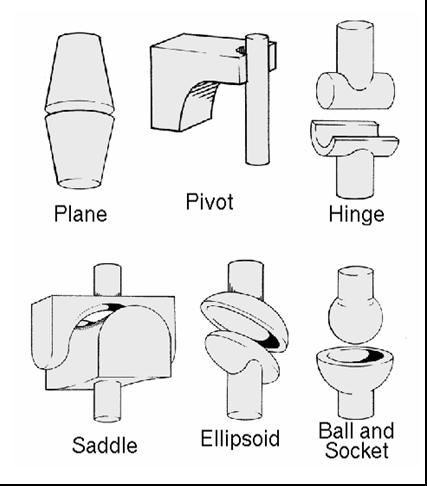
\includegraphics[scale=0.5]{imagens/fig2.jpg}
	\end{center}
    \caption{\label{fig_grafico}Descrição da imagem.}
\end{figure}

\subsection{Fundamentos 3}
\label{sec:fundamentos3}

\todo[inline]{Segue um exemplo de uso referências.}

Segundo \citeonline{knuth:84}, tem-se que $\dots$ \cite{boulic:91} e \cite{smith:99}.

\todo[inline]{Segue um exemplo de uso de referência de seção e de equações.}

Um exemplo de equação é apresentado na Equação~\ref{eq:poli}:

\begin{equation}
\label{eq:poli}
    f(n) = 4x^2 + 2y*12
\end{equation}

Outro exemplo de matemática em Latex: Calcule as raízes da equação $x^2 + 12x - 13 = 0$.
\begin{equation}
 x = \frac{-12 \pm \sqrt{12^2 - (4)(1)(-13)}}{(2)(1)} = \frac{-12 \pm \sqrt{196}}{2} = \frac{-12 \pm 14}{2} = -6 \pm 7
\end{equation}

%------------------------------------------
% Trabalho Relacionados
%------------------------------------------
\section{Trabalhos Relacionados}
\label{sec:trabalhos-re}


\todo[inline]{Nesta parte faz-se a revisão da literatura e do estado da prática sobre o assunto, analisando criticamente os resultados de estudos e soluções desenvolvidos por outros autores, cujas obras citadas e consultadas devem constar nas referências.}

\textcolor{red}{A função desta seção é demonstrar à banca que você conhece o estado da arte e o estado da prática do seu tema e que a lacuna identificada é real. O que faltar de conhecimento ou de solução é lacuna e, portanto, a oportunidade que você explora como problema de pesquisa. No mestrado, espera-se uma revisão estruturada e reprodutível: descreva brevemente o protocolo de busca adotado, isto é, as bases consultadas (por exemplo, IEEE Xplore, ACM Digital Library, Scopus, Web of Science e SBC OpenLib), a \textit{string} de busca, o período considerado e os critérios de inclusão e exclusão. Quando pertinente, conduza um mapeamento sistemático ou uma revisão sistemática da literatura. Priorize artigos de periódicos e conferências relevantes da área, preferencialmente dos últimos cinco anos, sem desconsiderar trabalhos seminais. O Google Acadêmico pode ser usado como fonte complementar.}

\textcolor{red}{As pesquisas que você irá buscar para compor esta seção são aquelas semelhantes à sua, ou seja, que investigam o mesmo tema e que atacam problemas de pesquisa nos quais você está interessado em estudar. Por se tratar de um Mestrado Profissional em Computação Aplicada, considere também o estado da prática: ferramentas, produtos e serviços existentes no mercado ou no setor público, soluções de código aberto, patentes e relatórios técnicos que tratem do mesmo problema no domínio de aplicação. Isso permite demonstrar por que as soluções existentes não atendem ao contexto real em que a sua pesquisa se insere.}

\textcolor{red}{A descrição de um estudo deve ocupar, idealmente, apenas um parágrafo. Como regra geral, um parágrafo pode ter até 20 linhas, mas tente trabalhar com o máximo de 12 ou 16. No máximo, a sua descrição de um estudo deve ocupar dois parágrafos, não mais que isso.}

\textcolor{red}{As descrições de estudos devem ser conectadas entre si por meio do texto. Ou seja, você pode afirmar que Santos (2022) investigou X e concluiu Y, sugerindo como trabalho futuro Z. Aí, no parágrafo seguinte, você pode dizer que Silva (2022), baseado em Santos (2022), conduziu estudo para investigar Z. Note, portanto, que os estudos foram, de algum modo, conectados no seu texto. Agrupe os trabalhos por abordagem, técnica ou subproblema, em vez de apresentá-los como uma lista isolada de resumos.}

\textcolor{red}{Como regra geral, a descrição de um estudo deve seguir o seguinte formato, que você pode adaptar: “Silva e Santos (2022) conduziram estudo cujo objetivo foi {Preencher com o verbo no infinitivo mais complemento adotado por Silva e Santos}. Para atingir esse objetivo, adotaram o seguinte método: {Preencher com uma breve descrição do método do estudo}. Os pesquisadores verificaram que {Preencher com os principais dados}. A partir desses dados, concluíram que {Preencher com a resposta à principal pergunta de pesquisa}. Esse estudo teve como principais limitações: {Preencher com uma breve síntese}. Em relação ao presente trabalho, {Preencher com a semelhança e a diferença em relação à sua proposta}”.}

\textcolor{red}{O parágrafo final desta seção deve explicitar a correlação entre as pesquisas e soluções descritas e, então, apresentar de modo inequívoco a lacuna, científica e/ou prática, que justifica o problema de pesquisa e a solução proposta apresentada na seção seguinte.}

\todo[inline]{Deve-se apresentar uma visão geral e comparativa dos trabalhos apresentados, indicando como cada trabalho pode contribuir com o seu. Sugere-se apresentar uma tabela comparativa entre os trabalhos, com critérios relevantes para o problema e o contexto de aplicação, incluindo uma linha para a sua proposta (``Este trabalho''), de modo a evidenciar o seu diferencial. Abaixo segue um exemplo:}

A seguir analisamos as técnicas (ver Tabela~\ref{Table:TechByPapers}) 
adotadas para a geração das invariantes de programa nos trabalhos apresentados anteriormente. Vale ressaltar que as técnicas identificadas foram:

\begin{itemize}
    \item \textbf{Análise de Predicados}. Analisando os métodos baseados na análise de predicado, podemos observar que a análise de predicado fornece um apoio significativo na análise do programa para inferir propriedades sobre o comportamento do programa;
    %
    \item \textbf{Interpretação Abstrata}. É uma teoria da aproximação da semântica de linguagens de programação cuja aplicação principal é a análise estática;
    %
    \item \textbf{Lógica de Mill}. A lógica de Mill é adotada para caracterizar laços por meio de uma função que define o seu espaço de estados.
    %
    \item \textbf{\textit{Templates}}. Analisando as publicações, notamos que a adoção de \textit{templates} é importante para fornecer um suporte para guiar a inferência de invariantes de programas.
\end{itemize}{}

%\multicolumn{number cols}{align}{text} % align: l,c,r
%\multirow{number rows}{width}{text}
\begin{table}[htbp]  
  \centering  
  \scalefont{0.9}  
  \begin{tabular}{|c|c|c|c|c|}
    \hline
    % header
    % row 1 and 2
    \multicolumn{1}{|c|}{\multirow{2}{*}{\textbf{Artigos}}} & 
    % row 1
    \multicolumn{4}{c|}{\textbf{Técnicas}} \bigstrut\\
    \cline{2-5} &
    % row 2
    \textbf{Predicados} & \textbf{Int. Abstrata} & \textbf{Log. Mill} & \textbf{\textit{Templates}} \bigstrut\\
    \hline
    % body table - row 3
    Trabalho 1 & X &  &  &  \bigstrut\\
    \hline
    % body table - row 4
    Trabalho 2 &  & X & X &  \bigstrut\\
    \hline
    % body table - row 5
    Trabalho 3 & X & X &  & X \bigstrut\\
    \hline
    % body table - row 6
    Trabalho 4 & X & X &  & X \bigstrut\\
    \hline
    % body table - row 7
    \textbf{Este trabalho} & X & X & X & X \bigstrut\\
    \hline
  \end{tabular}  
  \caption{Classificação dos artigos por técnicas.}
  \label{Table:TechByPapers}
\end{table}%

%--------------------------------------
% Solução Proposta
%--------------------------------------
\section{Solução Proposta}
\label{sec:solucao-proposta}


\todo[inline]{\textbf{NOTA}: Nesta seção, apresente a visão geral da solução proposta e os procedimentos metodológicos da pesquisa, com o instrumental, os métodos e as técnicas aplicados. No mestrado, caracterize a pesquisa quanto à natureza (aplicada), à abordagem (quantitativa, qualitativa ou mista), aos objetivos (exploratória, descritiva ou explicativa) e aos procedimentos técnicos (por exemplo, \textit{Design Science Research}, estudo de caso, pesquisa-ação ou experimento controlado), justificando cada escolha. Por se tratar de um Mestrado Profissional em Computação Aplicada, deixe explícito o contexto real de aplicação (organização, setor ou comunidade), os requisitos levantados junto aos usuários ou às partes interessadas e o produto técnico ou tecnológico que resultará da pesquisa. Como se trata do texto de qualificação, indique claramente o que já foi realizado e o que ainda será desenvolvido até a defesa. Caso a pesquisa envolva seres humanos ou dados pessoais, informe a submissão ao Comitê de Ética em Pesquisa (Plataforma Brasil) e as medidas de adequação à LGPD.}


%--------------------------------------
% Arquitetura
%--------------------------------------
\subsection{Arquitetura}

\todo[inline]{\textbf{NOTA}: Deve-se apresentar uma visão geral da solução proposta, por exemplo, usando uma \textit{Big Picture} que mostre a solução inserida no seu contexto de aplicação, com os usuários, os sistemas externos e os dados envolvidos. Abaixo segue um \textbf{exemplo}.} 

A Figura~\ref{fig_bigpicture} apresenta uma visão geral da solução proposta que visa o desenvolvimento e análise de um sistema de irrigação usando tecnologias de IoT.

\begin{figure}[h!]    
	\begin{center}
	    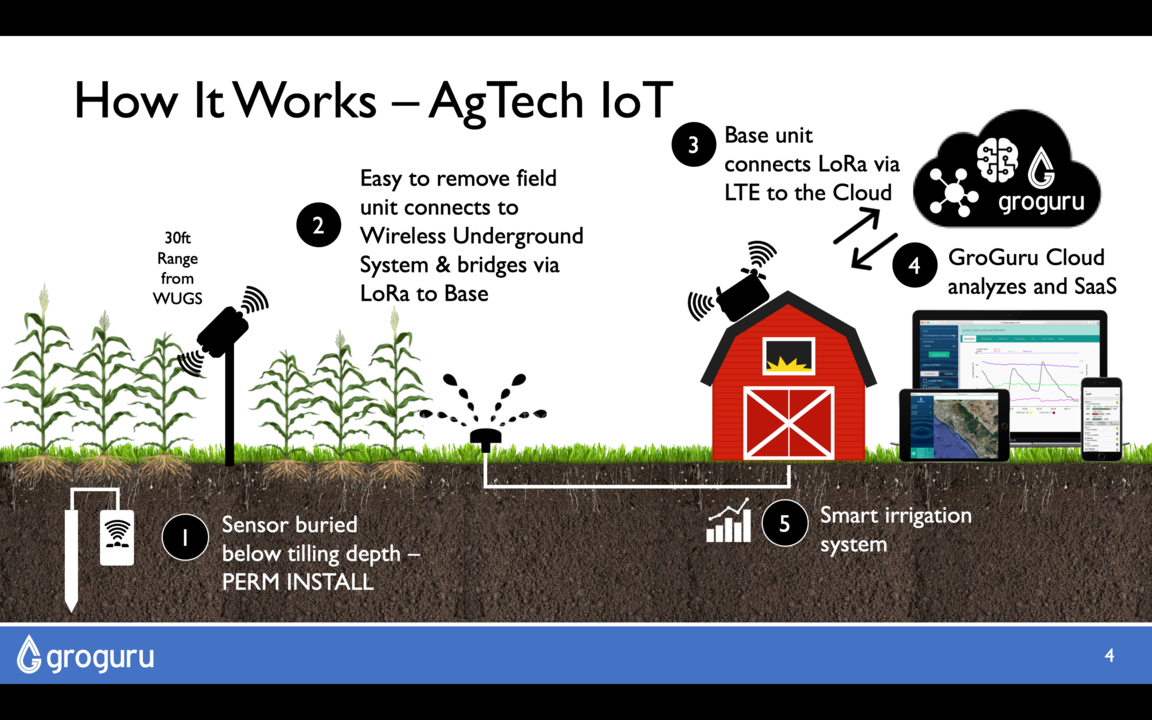
\includegraphics[scale=0.3]{imagens/bigpicture.png}
	\end{center}
	\caption{\label{fig_bigpicture}Como funciona o sistema de irrigação.}
\end{figure}

\todo[inline]{\textbf{NOTA}: Nesta seção, também deve-se apresentar o fluxo da sua solução, ou seja, um diagrama contendo os artefatos de entrada e saída para cada etapa da solução proposta. Um modelo de diagrama que pode ser utilizado é o BPMN (http://www.bpmn.org). Abaixo segue um \textbf{exemplo}.}

A Figura~\ref{fig_digflow} apresenta o fluxo de execução da solução proposta contendo suas respectivas entradas e artefatos gerados no modelo BPMN.

\begin{figure}[h!]	
	\begin{center}
	    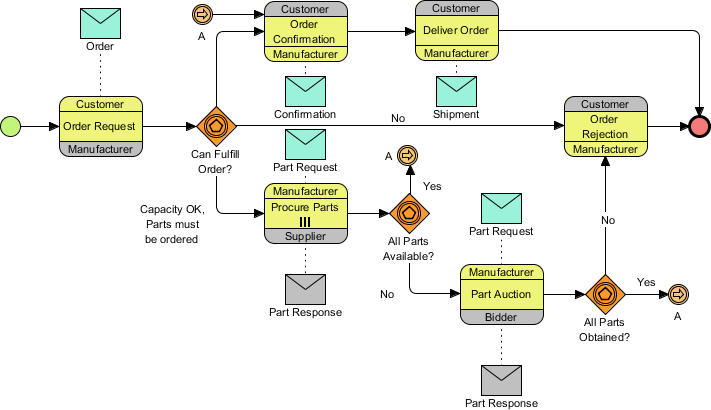
\includegraphics[scale=0.7]{imagens/34-final-business-process-diagram.png}
	\end{center}
    \caption{\label{fig_digflow}Diagrama de fluxo no modelo BPMN.}
\end{figure}


%--------------------------------------
% Modelagem e Análise
%--------------------------------------
\subsection{Modelagem e Análise}
\label{sec:modelagem-analise}

\todo[inline]{Nesta subseção, apresenta-se um panorama da arquitetura da solução, destacando os principais componentes, entidades e interações. Deve-se adotar pelo menos um tipo de modelagem, escolhido conforme a natureza do problema e justificado no texto. As subseções a seguir (UML, Autômatos Finitos, Redes de Petri e Análise de Corretude) são apenas exemplos: mantenha somente as que se aplicam ao seu trabalho e inclua outras, se necessário (por exemplo, modelagem de dados, arquitetura C4, modelos de aprendizado de máquina).}

\textcolor{red}{Exemplo: A solução proposta é composta por três módulos principais: (i) Interface do Usuário, (ii) Módulo de Processamento de Regras, e (iii) Gerenciador de Requisições. A comunicação entre os módulos é realizada por meio de eventos assíncronos. Para garantir a corretude das interações, utilizou-se modelagem formal com base em UML e Autômatos Finitos.}


\subsubsection{Modelagem com UML}

\textcolor{red}{Nesta parte, são apresentados os diagramas estruturais e comportamentais relevantes (e.g., casos de uso, atividades, estados, sequência, classes).}

\textcolor{red}{Exemplo:
%
A Figura 1 apresenta o Diagrama de Casos de Uso, onde é possível identificar os principais atores do sistema e suas interações com as funcionalidades.
A Figura 2 ilustra o Diagrama de Estados do componente Gerenciador de Requisições, evidenciando os estados "Inativo", "Aguardando Resposta" e "Erro de Timeout".}


\subsubsection{Modelagem com Autômatos Finitos}

\textcolor{red}{Aqui, são modelados formalmente os comportamentos dos módulos ou protocolos envolvidos, usando autômatos finitos determinísticos ou não determinísticos.}

\textcolor{red}{Exemplo:
%
O comportamento do módulo de autenticação foi modelado como um Autômato Finito Determinístico (AFD), conforme ilustrado na Figura 3.
O autômato possui os seguintes estados: q0 (esperando credenciais), q1 (verificação em andamento), q2 (acesso permitido), e q3 (acesso negado).
A transição de q0 para q1 ocorre ao receber um par usuário/senha; a transição para q2 ou q3 depende do resultado da verificação.}


\subsubsection{Modelagem com Redes de Petri}

\textcolor{red}{Utilize Redes de Petri para modelar e analisar aspectos concorrentes, sincronização e condições de deadlock.}

\textcolor{red}{Exemplo:
%
Para representar o processo de requisição e resposta entre cliente e servidor, modelamos o sistema utilizando uma Rede de Petri (Figura 4).
A rede inclui lugares como ClientePronto, RequisiçãoEnviada, ServidorOcupado e transições como EnviarRequisição, ProcessarRequisição, e ResponderCliente.
Foi verificada a ausência de deadlocks e a reentrância do sistema, assegurando que sempre será possível retornar ao estado inicial após uma interação completa.}


\subsubsection{Análise de Corretude}

\todo[inline]{\textbf{NOTA}: Aqui, discute-se os limites da modelagem, possíveis extensões e como os resultados reforçam a confiança na solução.}

\textcolor{red}{Apresente aqui os critérios de análise formal e os resultados obtidos com base nos modelos apresentados. Você pode usar ferramentas de verificação (ex: SPIN, TINA, NuSMV, UPPAAL) ou provas matemáticas.
%
Exemplo: A partir do modelo em autômatos, foi possível aplicar a verificação de propriedades de segurança e vivacidade.
Utilizando a ferramenta NuSMV, especificamos as propriedades desejadas em LTL (Linear Temporal Logic), como: $G(request -> F(response))$ - toda requisição será eventualmente respondida; $G \neg deadlock$ - ausência de deadlock em qualquer execução do sistema.
Todas as propriedades foram verificadas satisfatoriamente, confirmando a corretude formal da solução.}

\textcolor{red}{A modelagem revelou potenciais condições de corrida entre os módulos de log e autenticação, levando à introdução de um mecanismo adicional de controle de concorrência.
A utilização de três diferentes abordagens formais (UML, Autômatos, e Redes de Petri) permitiu uma análise multifacetada do sistema, contemplando tanto aspectos estruturais quanto comportamentais.}


\subsection{Ambiente de Desenvolvimento e Implementação da Solução}

\todo[inline]{\textbf{NOTA}: Deve-se apresentar as ferramentas adotadas na solução proposta e explicar como elas se relacionam. \textbf{Importante}: mencione o nome da ferramenta, a versão e onde pode ser encontrada, de modo a garantir a reprodutibilidade. Descreva também o estágio atual da implementação (protótipo, versão funcional, implantação piloto), o repositório do código-fonte e a licença adotada. Segue um pequeno \textbf{exemplo}.}

\textcolor{red}{Exemplo: A solução proposta será uma ferramenta de verificação de código implementada como um transformador de código escrita em C/C++ usando o \textit{framework} para compiladores LLVM~\footnote{https://llvm.org/} (v$6.0$). A solução utilizará como \textit{front-end} para programas escritos em C o Clang~\footnote{https://clang.llvm.org/} (v$6.0$) para gerar código LLVM-bitcode que será usado para a transformação de código. As ferramentas LibFuzzer (v$6.0$) e KLEE (v$2.0$) serão utilizadas para gerar entrada de testes para os códigos que serão analisados. Finalmente, o MetaSMT (v$4.rc2$) será usado como API para motores de resolvedores de satisfatibilidade.}


\subsection{Produto Técnico ou Tecnológico}
\label{sec:produto-tecnico}

\todo[inline]{\textbf{NOTA}: No Mestrado Profissional, a pesquisa deve resultar em um produto técnico ou tecnológico (por exemplo, software ou aplicativo, processo ou tecnologia, base de dados, protocolo, manual ou relatório técnico), que é considerado na avaliação dos programas pela CAPES. Descreva o produto esperado, o seu tipo, o público-alvo ou a organização beneficiada, o grau de inovação e o impacto esperado, bem como a forma de disponibilização e de validação no contexto real de aplicação. Consulte o Regimento Interno do PPCA para verificar as exigências específicas do programa quanto ao produto.}

%------------------------------------------
% Avaliação Experimental
%------------------------------------------
\section{Avaliação Experimental}
\label{sec:plan-experimentos}


\todo[inline]{\textbf{NOTA}: Deve-se adicionar um texto para introduzir a seção. No texto de qualificação, esta seção deve apresentar o planejamento completo da avaliação e, quando houver, os resultados preliminares já obtidos, permitindo que a banca avalie a viabilidade e o rigor da avaliação antes da sua execução final. Segue um \textbf{exemplo}.}

Esta seção descreve o planejamento da avaliação experimental da solução proposta, incluindo o projeto do estudo empírico que será executado para avaliá-la, bem como os resultados preliminares obtidos até o momento.


\subsection{Projeto da Avaliação Experimental}
\label{sub:experimento}

\todo[inline]{\textbf{NOTA}: Deve-se descrever o projeto da avaliação da solução proposta, incluindo o objetivo, o ambiente, os elementos utilizados, os artefatos de entrada e saída, os dados coletados e as métricas de avaliação. Recomenda-se estruturar o objetivo com o paradigma GQM (\textit{Goal-Question-Metric}), associando cada questão de pesquisa a métricas objetivas, e definir as \textit{baselines} com as quais a solução será comparada (por exemplo, os trabalhos relacionados ou a prática atual da organização). Por se tratar de um Mestrado Profissional em Computação Aplicada, a avaliação deve contemplar, sempre que possível, a validação no contexto real de aplicação, com usuários, dados ou processos da organização ou do setor beneficiado (por exemplo, estudo de caso, implantação piloto, avaliação de usabilidade ou de aceitação da tecnologia). Caso a avaliação envolva seres humanos, informe a aprovação no Comitê de Ética em Pesquisa (Plataforma Brasil). Segue um \textbf{exemplo} abaixo.}

\textcolor{red}{Esta seção descreve o planejamento e o projeto de um estudo empírico com o objetivo de avaliar a solução proposta para \textcolor{red}{XXXXX}. O estudo será conduzido aplicando a solução proposta sobre \textit{benchmarks} públicos de programas em C e sobre programas fornecidos pela organização parceira \textcolor{red}{XXXXX}. Os experimentos serão executados em um computador Intel Xeon CPU E5, 2.60GHz, 115GB RAM com Linux 3.13.0-35-generic x86\_64.}

\todo[inline]{\textbf{NOTA}: Deve-se também apresentar como a avaliação será executada e qual o objetivo de cada ação. Neste momento você deve considerar os cenários de teste mais importantes e a forma de coleta e de análise dos dados, incluindo os testes estatísticos, quando aplicáveis. Segue um \textbf{exemplo}.}

\textcolor{red}{Esta avaliação empírica tem como objetivo analisar a capacidade do método proposto, sobre \textit{benchmarks} públicos de programas em C, de contribuir com a verificação executada pelo software $X$. Desta forma, nesta avaliação, investigam-se as seguintes questões de pesquisa (QP):
%
\begin{itemize}
    \item[QP1]: As ferramentas para a geração de invariantes são capazes de suportar as diferentes estruturas da linguagem de programação C?
    %
    \item[QP2]: As abordagens propostas para geração de dados de teste contribuem para a geração de invariantes?
    %
    \item[QP3]: As invariantes geradas contribuem para a verificação executada pelo ESBMC?
    %
    \item[QP4]: A solução proposta é aplicável ao processo de desenvolvimento da organização parceira, na percepção dos seus usuários?
\end{itemize}}


\todo[inline]{\textbf{NOTA}: Deve-se também apresentar as etapas da experimentação e o cronograma de execução, indicando quais etapas já foram concluídas e quais serão realizadas até a defesa.}


\subsection{Resultados Preliminares}
\label{sub:analise-resultados}

\todo[inline]{\textbf{NOTA}: No texto de qualificação, apresente os resultados preliminares obtidos até o momento (por exemplo, de um estudo piloto, de uma prova de conceito ou da execução parcial dos experimentos), deixando claro o seu caráter parcial. Caso ainda não haja resultados, descreva como os resultados serão analisados e discutidos. As orientações abaixo valem tanto para os resultados preliminares quanto para os resultados finais, a serem apresentados na dissertação.}

\textcolor{red}{A função desta seção é apresentar os produtos e/ou dados obtidos após a execução da solução proposta, bem como a interpretação desses dados a partir da teoria, seguida pelo apontamento das respostas às perguntas de pesquisa. Tais respostas precisam ser comparadas com o conhecimento científico existente, de modo que o leitor perceba em que medida se aproximam ou se distanciam do que já era conhecido. Por se tratar de um Mestrado Profissional, discuta também as implicações práticas dos resultados para a organização ou o setor beneficiado.}

\textcolor{red}{Lembre-se que discutir um resultado, geralmente, significa: 1. Comparar o seu dado ou resposta com a literatura descrita na seção de Trabalhos Relacionados, apontando se o resultado foi convergente ou divergente com outros dados observados na literatura; 2. Explicar o resultado com base na literatura descrita na seção de Fundamentos Teóricos, o que significa dizer se o resultado era esperado ou não. E, quando isso não for possível, levantar hipóteses que expliquem o resultado; 3. Indicar as implicações do resultado para pesquisas futuras e para a prática profissional; 4. Descrever o que significa o resultado, esclarecendo para o leitor, por exemplo, se o dado é um bom indicador ou não em relação ao que está se tentando responder na pesquisa.}

\textcolor{red}{Ao apresentar tabelas e figuras, não se limite a repetir o que já está nesses elementos gráficos. Destaque a principal informação de uma tabela ou figura, aquela à qual o leitor não pode deixar de prestar atenção, ou resuma o principal achado referente a ela. Sempre adote o seguinte modelo: primeiro apresente a tabela ou figura {“A Tabela 1 exibe…”}, depois coloque o elemento gráfico e, por fim, comente o que há de principal nele.}


\subsection{Ameaças à Validade}
\label{sub:ameacas-validade}

\textcolor{red}{Aponte as limitações do estudo, isto é, os fatores que podem comprometer a confiabilidade e a generalidade das respostas às perguntas de pesquisa, e as estratégias adotadas para mitigá-los. Recomenda-se organizar a discussão em ameaças à validade interna, externa, de construção e de conclusão. Por exemplo: o uso de \textit{benchmarks} públicos pode não representar os programas da organização parceira (validade externa), o que será mitigado pela inclusão de programas reais fornecidos por ela.}

%------------------------------------------
% Considerações Finais
%------------------------------------------
\section{Considerações Finais}
\label{sec:conclusao}


\todo[inline]{\textbf{NOTA}: No texto de qualificação, as considerações finais têm caráter parcial e devem permitir que a banca avalie o andamento da pesquisa e a viabilidade de concluí-la no prazo regimental do mestrado. Descreva, de forma resumida: (1) o que já foi desenvolvido, relacionando-o aos objetivos específicos; (2) os resultados preliminares e as contribuições esperadas, tanto científicas quanto o produto técnico ou tecnológico e o seu impacto no contexto de aplicação; (3) os riscos e os desafios para as próximas etapas, com as respectivas estratégias de mitigação; e (4) o cronograma das atividades até a defesa da dissertação. Exemplo abaixo:}

\textcolor{red}{O objetivo deste estudo é [PREENCHER]. Para alcançá-lo, adota-se [PREENCHER COM UMA SÍNTESE DE DUAS A TRÊS LINHAS SOBRE O MÉTODO]. Até o momento, foram concluídas as seguintes etapas: [PREENCHER COM AS ATIVIDADES REALIZADAS E OS OBJETIVOS ESPECÍFICOS JÁ ATENDIDOS]. Os resultados preliminares indicam que [PREENCHER COM A SÍNTESE DOS RESULTADOS PRELIMINARES E COM O QUE ELES SUGEREM EM RELAÇÃO À PERGUNTA DE PESQUISA].}

\textcolor{red}{Como contribuições esperadas, destacam-se [PREENCHER COM AS CONTRIBUIÇÕES CIENTÍFICAS] e o desenvolvimento de [PREENCHER COM O PRODUTO TÉCNICO OU TECNOLÓGICO], que deverá beneficiar [PREENCHER COM A ORGANIZAÇÃO, O SETOR OU O PÚBLICO-ALVO]. Como próximas etapas, pretende-se [PREENCHER COM AS ATIVIDADES PENDENTES]. Os principais desafios identificados são [PREENCHER COM OS RISCOS, POR EXEMPLO, ACESSO A DADOS OU A USUÁRIOS DA ORGANIZAÇÃO PARCEIRA], que serão mitigados por meio de [PREENCHER COM AS ESTRATÉGIAS DE MITIGAÇÃO].}

\textcolor{red}{Pretende-se, ainda, submeter os resultados da pesquisa a [PREENCHER COM OS PERIÓDICOS OU CONFERÊNCIAS-ALVO] e registrar ou disponibilizar o produto desenvolvido por meio de [PREENCHER, POR EXEMPLO, REGISTRO DE SOFTWARE NO INPI OU REPOSITÓRIO PÚBLICO].}


\subsection{Cronograma}
\label{sub:cronograma}

\todo[inline]{\textbf{NOTA}: Apresente o cronograma das atividades a serem realizadas entre a qualificação e a defesa, compatível com o prazo regimental do PPCA. Ajuste as atividades e os meses ao seu trabalho. Segue um \textbf{exemplo}.}

A Tabela~\ref{tab:cronograma} apresenta o cronograma das atividades previstas até a defesa da dissertação.

\begin{table}[htbp]
  \centering
  \scalefont{0.9}
  \begin{tabular}{|l|c|c|c|c|c|c|}
    \hline
    \multicolumn{1}{|c|}{\multirow{2}{*}{\textbf{Atividades}}} & \multicolumn{6}{c|}{\textbf{Meses}} \bigstrut\\
    \cline{2-7}
    & \textbf{1} & \textbf{2} & \textbf{3} & \textbf{4} & \textbf{5} & \textbf{6} \bigstrut\\
    \hline
    Ajustes sugeridos pela banca de qualificação & X &  &  &  &  &  \bigstrut\\
    \hline
    Implementação do produto técnico ou tecnológico & X & X & X &  &  &  \bigstrut\\
    \hline
    Execução da avaliação experimental &  &  & X & X &  &  \bigstrut\\
    \hline
    Análise dos resultados &  &  &  & X & X &  \bigstrut\\
    \hline
    Submissão de artigo científico &  &  &  &  & X &  \bigstrut\\
    \hline
    Escrita da dissertação &  & X & X & X & X & X \bigstrut\\
    \hline
    Defesa da dissertação &  &  &  &  &  & X \bigstrut\\
    \hline
  \end{tabular}
  \caption{Cronograma das atividades até a defesa.}
  \label{tab:cronograma}
\end{table}



%--------------------------------------
% Referências
%--------------------------------------
\addcontentsline{toc}{section}{Referências}
\bibliography{referencias}


%--------------------------------------
% Anexos
%--------------------------------------
% Capa personalizada para UFRR
\begin{center}        
    \vspace*{\fill}
    {\Huge \textbf{ANEXOS}}\\
    \vspace*{\fill}
\end{center}

%------------------------------------------
% Título: Anexo 01 - Termo de responsabilidade do discente
%------------------------------------------
\section*{ANEXO 01 - TERMO DE RESPONSABILIDADE DO DISCENTE}
\addcontentsline{toc}{section}{ANEXO 01 - TERMO DE RESPONSABILIDADE DO DISCENTE}
\label{sec:anexo-1}

\vspace*{\fill}

Pelo presente TERMO DE RESPONSABILIDADE, eu, \textbf{XXXXXXXX}, sob o número de matrícula \textbf{XXXXXXXX}, discente do Mestrado Profissional do Programa de Pós-Graduação em Computação Aplicada (PPCA) da Universidade Federal de Roraima (UFRR), comprometo-me a participar das atividades de orientação pertinentes ao desenvolvimento da pesquisa de mestrado nos dias e horários agendados e acordados com o(a) meu(minha) orientador(a), \getorientador, e responsabilizo-me pela autenticidade e originalidade do texto submetido ao Exame de Qualificação, bem como da dissertação e dos produtos técnicos e tecnológicos dela decorrentes.

Declaro ter conhecimento de que a ausência injustificada às atividades de orientação e o não cumprimento dos prazos estabelecidos pelo programa poderão acarretar meu desligamento do PPCA, nos termos de seu Regimento Interno.

Aceito e comprometo-me a cumprir as normas do Regimento Interno do PPCA e as demais normas de pós-graduação \textit{stricto sensu} da UFRR, inclusive quanto ao prazo para realização do Exame de Qualificação e da defesa da dissertação, e a não abandonar a pesquisa, salvo por motivo justificado, a ser apreciado pelo Colegiado do Programa.

Por fim, comprometo-me a observar as orientações recebidas; a zelar pela integridade científica, atribuindo a devida autoria às ideias, aos textos e aos dados de terceiros; e a buscar qualidade, rigor metodológico e aplicabilidade prática nos resultados da pesquisa.

\vspace*{\fill}

\begin{center}
    Boa Vista, \textbf{XXXXXXXX} de \textbf{XXXXXXXX} de \textbf{XXXXXXXX}. \\[1.0cm]
    \rule{7cm}{0.4pt} \\
    \fontsize{12}{15}\selectfont Assinatura do Orientando
\end{center}


\vfill


%------------------------------------------
% ANEXO 02 - DECLARAÇÃO DE AUTORIA
%------------------------------------------
\section*{ANEXO 02 - DECLARAÇÃO DE AUTORIA}
\addcontentsline{toc}{section}{ANEXO 02 - DECLARAÇÃO DE AUTORIA}
\label{sec:anexo-2}


\begin{center}
    \fontsize{12}{15}\selectfont
    \vspace*{0.5cm}
    \textbf{DECLARAÇÃO DE AUTORIA}
    \vspace*{1cm}
\end{center}

\vspace*{\fill}

Eu, \textbf{Nome completo do discente} (código de matricula \textbf{0000000000}), discente do Mestrado Profissional do Programa de Pós-Graduação em Computação Aplicada (PPCA) da Universidade Federal de Roraima (UFRR) e autor(a) do texto de qualificação de mestrado intitulado \textbf{ ... }, declaro que o trabalho em referência é de minha autoria, desenvolvido sob a orientação de \getorientador, e que é de minha inteira responsabilidade o texto apresentado à banca do Exame de Qualificação. Declaro, ainda, que as citações diretas e indiretas, os dados, as figuras e os demais conteúdos de terceiros, inclusive de trabalhos meus já publicados, estão devidamente referenciados com as respectivas obras e anos de publicação. Declaro, para os devidos fins, que estou ciente:
\begin{itemize}\setlength\itemsep{.02em}
    \item  dos Artigos 297 a 299 do Código Penal, Decreto-Lei n. 2.848 de 7 de dezembro de 1940;
    %
    \item  da Lei n. 9.610, de 19 de fevereiro de 1998, sobre os Direitos Autorais; e
    %
    \item  que plágio consiste na reprodução de obra alheia e submissão da mesma como trabalho próprio ou na inclusão, em trabalho próprio, de ideias, textos, tabelas ou ilustrações (quadros, figuras, gráficos, fotografias, retratos, lâminas, desenhos, organogramas, fluxogramas, plantas, mapas e outros) transcritos de obras de terceiros sem a devida e correta citação da referência.
\end{itemize}

A banca examinadora do Exame de Qualificação poderá não aceitar o referido trabalho caso os pontos mencionados acima sejam descumpridos, considerando-me, por conseguinte, reprovado(a) no exame, sem prejuízo das demais sanções previstas no Regimento Interno do PPCA e na legislação vigente.

\vspace*{\fill}

\begin{center}
    \rule{7cm}{0.4pt} \\
    \fontsize{12}{15}\selectfont Assinatura do acadêmico(a) \\ 
    Boa Vista - RR, data (por extenso).
\end{center}

\vfill


\end{document}
